\documentclass[12pt,a4paper]{article}
\usepackage[utf8]{inputenc}
\usepackage[T1]{fontenc}
\usepackage{amsmath}
\usepackage{amsfonts}
\usepackage{amssymb}
\usepackage{graphicx}
\usepackage[width=0.00cm, left=3.00cm, right=2.00cm, top=3.00cm, bottom=2.00cm]{geometry}
\usepackage{booktabs}
\usepackage{pgfplots}
\usepackage{adjustbox}
\title{Lista 3}
\usepackage{multirow}
\date{}
\begin{document}
	\begin{center}
		\includegraphics[width=100px]{Logo.png}\\
		\textsc{Universidade Federal de Pernambuco\\
			Centro de Ciências Sociais Aplicadas\\
			Departamento de Ciências Contábeis e Atuariais\\}
		\vspace{5cm}
		\huge Lista 3\\ \normalsize
		\vspace{4cm}
		Thales Rousseau Braga Reis Silva
	\end{center}
	\newpage
	\textbf{1. Laringe}
	\vspace{0.5cm}\\
	Um estudo clínico realizado com 90 pacientes  do sexo masculino diagnosticados com câncer de laringe. Os dados coletados foram idade dos pacientes no diagnóstico, estágio da doença; (I = Tumor primário - 33 pacientes, II = Envolvimento dos nódulos - 17 pacientes, III = Metástase - 27 pacientes e IV = Combinações dos estágios anteriores - 13 pacientes), além do tempo de acompanhamento e presença de censura.
	\vspace{0.5cm}
	\begin{center}
		\small{Tabela 1: Tempos de sobrevivência observados no estudo de câncer de laringe  - Grupo 1}
		\begin{tabular}{|c|c|c|}\hline
			\textbf{Estágio} & \textbf{Idade} & \textbf{Tempo de Acompanhamento}\\ \hline
			\multirow{33}{*}{I} & 43 & 3.5+\\ \cline{2-3}
			& 45 & 2.4+\\ \cline{2-3}
			& 47  & 5.9\\ \cline{2-3}
			& 48  & 4.5\\ \cline{2-3}
			& 51  & 3.2\\ \cline{2-3}
			& 52 & 4.0+\\ \cline{2-3}
			& 53 & 1.3+\\ \cline{2-3}
			& 56  & 8.1\\ \cline{2-3}
			& 57  & 2.5\\ \cline{2-3}
			& 58 & 3.2+\\ \cline{2-3}
			& 58  & 5.9\\ \cline{2-3}
			& 58  & 9.6\\ \cline{2-3}
			& 60 & 3.5+\\ \cline{2-3}
			& 61  & 6.6\\ \cline{2-3}
			& 63 & 4.0+\\ \cline{2-3}
			& 63  & 3.3\\ \cline{2-3}
			& 64  & 6.2\\ \cline{2-3}
			& 66  & 7.0\\ \cline{2-3}
			& 67 & 6.5+\\ \cline{2-3}
			& 68 & 7.4+\\ \cline{2-3}
			& 68  & 4.5\\ \cline{2-3}
			& 68  & 10.7\\ \cline{2-3}
			& 70  & 5.5\\ \cline{2-3}
			& 73  & 7.4\\ \cline{2-3}
			& 73  & 8.1\\ \cline{2-3}
			& 75 & 6.0+\\ \cline{2-3}
			& 76 & 3.3+\\ \cline{2-3}
			& 77 & 0.6+\\ \cline{2-3}
			& 77 & 6.+\\ \cline{2-3}
			& 77  & 6.1\\ \cline{2-3}
			& 79  & 6.5\\ \cline{2-3}
			& 81 & 5.3+\\ \cline{2-3}
			& 86 & 4.3+\\ \hline
		\end{tabular}
		\vspace{1cm}\\
		\small{Tabela 2: Tempos de sobrevivência observados no estudo de câncer de laringe  - Grupo 2}
		\begin{tabular}{|c|c|c|}\hline
			\textbf{Estágio} & \textbf{Idade} & \textbf{Tempo de Acompanhamento}\\ \hline
			\multirow{16}{*}{II} & 47 & 4.3\\ \cline{2-3}
			& 50 & 7.5\\ \cline{2-3}
			& 51 & 3.3\\ \cline{2-3}
			& 53 & 7.6\\ \cline{2-3}
			& 61 & 9.3\\ \cline{2-3}
			& 62 & 7.0+\\ \cline{2-3}
			& 63 & 2.0+\\ \cline{2-3}
			& 64 & 1.8+\\ \cline{2-3}
			& 64 & 4.3\\ \cline{2-3}
			& 66 & 5.0\\ \cline{2-3}
			& 67 & 2.6\\ \cline{2-3}
			& 70 & 3.6+\\ \cline{2-3}
			& 71 & 6.2\\ \cline{2-3}
			& 72 & 3.6\\ \cline{2-3}
			& 74 & 2.2+\\ \cline{2-3}
			& 81 & 4.0+\\ \cline{2-3}
			& 86 & 0.2+\\ \hline
		\end{tabular}
		\vspace{1cm}\\
		\small{Tabela 3: Tempos de sobrevivência observados no estudo de câncer de laringe  - Grupo 3}
		\begin{tabular}{|c|c|c|}\hline
			\textbf{Estágio} & \textbf{Idade} & \textbf{Tempo de Acompanhamento}\\ \hline
			\multirow{27}{*}{III} & 49 & 0.3+\\ \cline{2-3}
			& 49 & 1.0+\\ \cline{2-3}
			& 49 & 5.0\\ \cline{2-3}
			& 51 & 10.1\\ \cline{2-3}
			& 52 & 3.7\\ \cline{2-3}
			& 53 & 1.9+\\ \cline{2-3}
			& 54 & 3.2+\\ \cline{2-3}
			& 54 & 4.8\\ \cline{2-3}
			& 57 & 0.5+\\ \cline{2-3}
			& 59 & 5.0+\\ \cline{2-3}
			& 60 & 1.3+\\ \cline{2-3}
			& 63 & 4.8\\ \cline{2-3}
			& 64 & 1.6+\\ \cline{2-3}
			& 65 & 6.4+\\ \cline{2-3}
			& 65 & 6.5\\ \cline{2-3}
			& 66 & 4.5\\ \cline{2-3}
			& 68 & 7.8+\\ \cline{2-3}
			& 69 & 5.1\\ \cline{2-3}
			& 69 & 9.3\\ \cline{2-3}
			& 70 & 6.3+\\ \cline{2-3}
			& 71 & 0.3+\\ \cline{2-3}
			& 72 & 1.9+\\ \cline{2-3}
			& 74 & 1.8+\\ \cline{2-3}
			& 78 & 8.0\\ \cline{2-3}
			& 79 & 0.7+\\ \cline{2-3}
			& 81 & 3.5+\\ \cline{2-3}
			& 82 & 0.8+\\ \hline			
		\end{tabular}
		\vspace{1cm}\\
		\small{Tabela 3: Tempos de sobrevivência observados no estudo de câncer de laringe  - Grupo 4}
		\begin{tabular}{|c|c|c|}\hline
			\textbf{Estágio} & \textbf{Idade} & \textbf{Tempo de Acompanhamento}\\ \hline
			\multirow{13}{*}{IV} & 41 & 1.0+\\ \cline{2-3}
			& 48 & 4.3\\ \cline{2-3}
			& 62 & 2.3+\\ \cline{2-3}
			& 65 & 0.1+\\ \cline{2-3}
			& 65 & 0.8+\\ \cline{2-3}
			& 68 & 1.5+\\ \cline{2-3}
			& 69 & 2.0+\\ \cline{2-3}
			& 71 & 0.3+\\ \cline{2-3}
			& 71 & 3.6+\\ \cline{2-3}
			& 74 & 2.9\\ \cline{2-3}
			& 76 & 0.4+\\ \cline{2-3}
			& 78 & 0.8+\\ \cline{2-3}
			& 84 & 3.8+\\ \hline
		\end{tabular}
	\end{center}
	\vspace{2cm}
	\textbf{2. Histograma dos dados}
	\begin{center}
		\vspace{1cm}
		\textbf{Histograma de Eventos - Grupo 1}
		\resizebox{300px}{!}{
			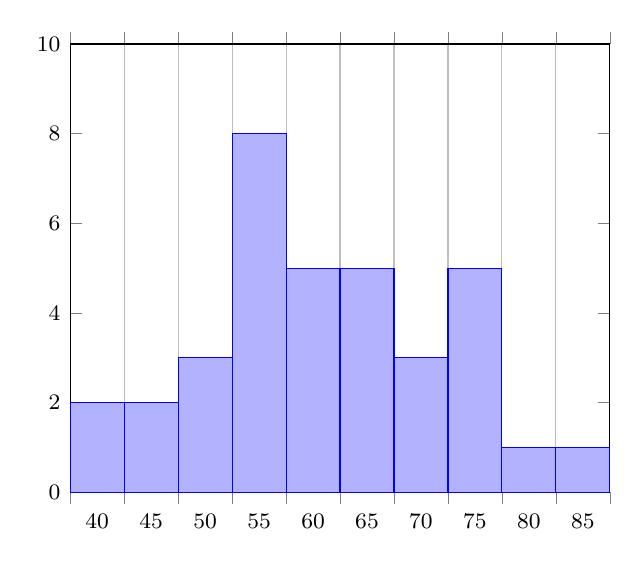
\begin{tikzpicture}
			\tikzstyle{every node}=[font=\footnotesize]
			\begin{axis}[ybar interval, ymin=0, ymax=10, xmin=40, xmax=90]
			\addplot coordinates {(40,2) (45,2) (50,3) (55,8) (60,5) (65,5) (70,3) (75,5) (80,1) (85,1) (90,0)};
			\end{axis}
			\end{tikzpicture}
		}
		\vspace{1cm}\\
		\textbf{Histograma de Sobrevivência - Grupo 1}
		\resizebox{300px}{!}{
			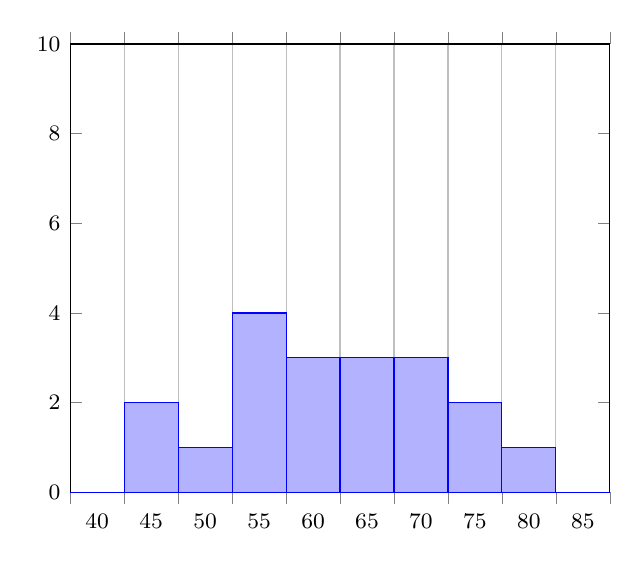
\begin{tikzpicture}
			\tikzstyle{every node}=[font=\footnotesize]
			\begin{axis}[ybar interval, ymin=0, ymax=10, xmin=40, xmax=90]
			\addplot coordinates {(40,0) (45,2) (50,1) (55,4) (60,3) (65,3) (70,3) (75,2) (80,1) (85,0) (90,0)};
			\end{axis}
			\end{tikzpicture}
		}
		\vspace{1cm}\\
		\textbf{Histograma de Censuras - Grupo 1}
		\resizebox{300px}{!}{
			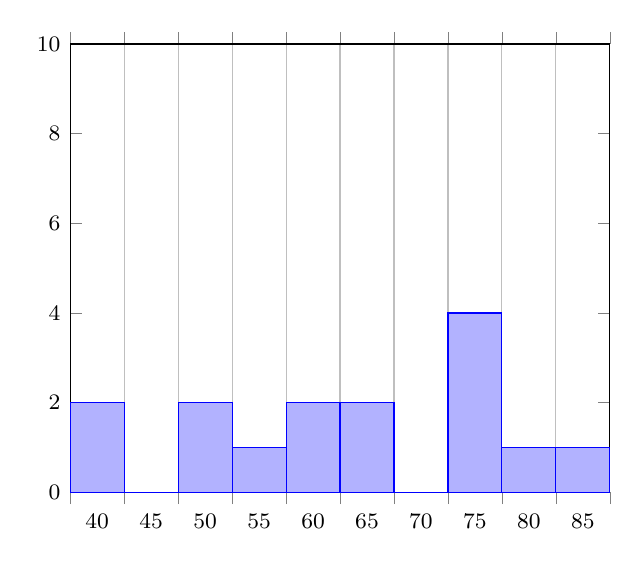
\begin{tikzpicture}
			\tikzstyle{every node}=[font=\footnotesize]
			\begin{axis}[ybar interval, ymin=0, ymax=10, xmin=40, xmax=90]
			\addplot coordinates {(40,2) (45,0) (50,2) (55,1) (60,2) (65,2) (70,0) (75,4) (80,1) (85,1) (90,0)};
			\end{axis}
			\end{tikzpicture}
		}
		\end{center}
		\vspace{1cm}
		Os dados do grupo com Estágio I de câncer de laringe quando analisado em formato histograma, as observações ficam concentrados na porção central, entre as idades de 55 e 75 anos. Esse padrão ocorre pela de presença do evento morte dos pacientes entre essas faixas etárias, já que os dados de censura se distribuem uniformemente entre as todas as idades.
		\vspace{2cm}\\
		\begin{center}
		\textbf{Histograma de Eventos - Grupo 2}
		\resizebox{300px}{!}{
			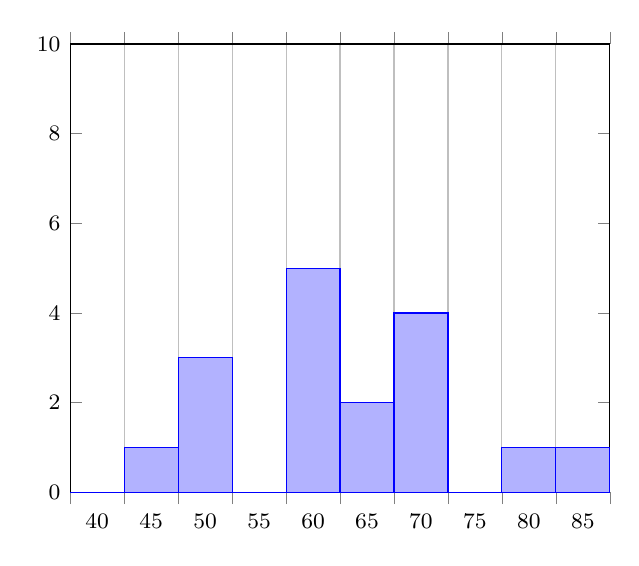
\begin{tikzpicture}
			\tikzstyle{every node}=[font=\footnotesize]
			\begin{axis}[ybar interval, ymin=0, ymax=10, xmin=40, xmax=90]
			\addplot coordinates {(40,0) (45,1) (50,3) (55,0) (60,5) (65,2) (70,4) (75,0) (80,1) (85,1) (90,0)};
			\end{axis}
			\end{tikzpicture}
		}
		\vspace{1cm}\\
		\textbf{Histograma de Sobrevivência - Grupo 2}
		\resizebox{300px}{!}{
			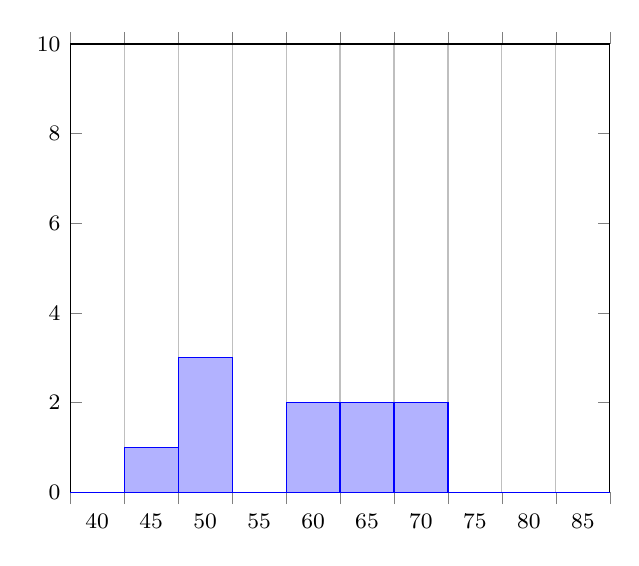
\begin{tikzpicture}
			\tikzstyle{every node}=[font=\footnotesize]
			\begin{axis}[ybar interval, ymin=0, ymax=10, xmin=40, xmax=90]
			\addplot coordinates {(40,0) (45,1) (50,3) (55,0) (60,2) (65,2) (70,2) (75,0) (80,0) (85,0) (90,0)};
			\end{axis}
			\end{tikzpicture}
		}
		\vspace{1cm}\\
		\textbf{Histograma de Censuras - Grupo 2}
		\resizebox{300px}{!}{
			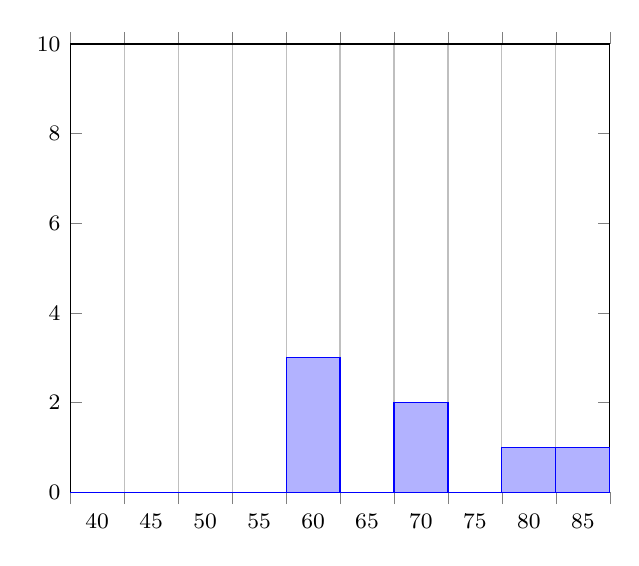
\begin{tikzpicture}
			\tikzstyle{every node}=[font=\footnotesize]
			\begin{axis}[ybar interval, ymin=0, ymax=10, xmin=40, xmax=90]
			\addplot coordinates {(40,0) (45,0) (50,0) (55,0) (60,3) (65,0) (70,2) (75,0) (80,1) (85,1) (90,0)};
			\end{axis}
			\end{tikzpicture}
		}
		\end{center}
		\vspace{1cm}
		As observações do grupo de pacientes com Estágio II de câncer de laringe, embora se concentrem levemente ao centro. Assim, analisando o histograma de ocorrência do evento morte, as observações parecem acontecer de maneira constante entre as faixas etárias até 75 anos, enquanto os eventos de censura ocorrem a partir dos 60 anos, assim ao visualizar o histograma geral, essas duas curvas se sobrepõem criando a maior ocorrência de eventos no centro do histograma.
		\vspace{2cm}\\
		\begin{center}
		\textbf{Histograma de Eventos - Grupo 3}
		\resizebox{300px}{!}{
			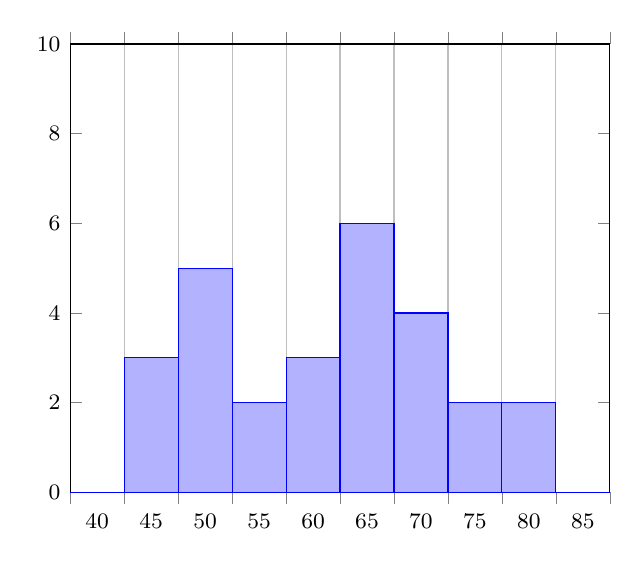
\begin{tikzpicture}
			\tikzstyle{every node}=[font=\footnotesize]
			\begin{axis}[ybar interval, ymin=0, ymax=10, xmin=40, xmax=90]
			\addplot coordinates {(40,0) (45,3) (50,5) (55,2) (60,3) (65,6) (70,4) (75,2) (80,2) (85,0) (90,0)};
			\end{axis}
			\end{tikzpicture}
		}
		\vspace{1cm}\\
		\textbf{Histograma de Sobrevivência - Grupo 3}
		\resizebox{300px}{!}{
			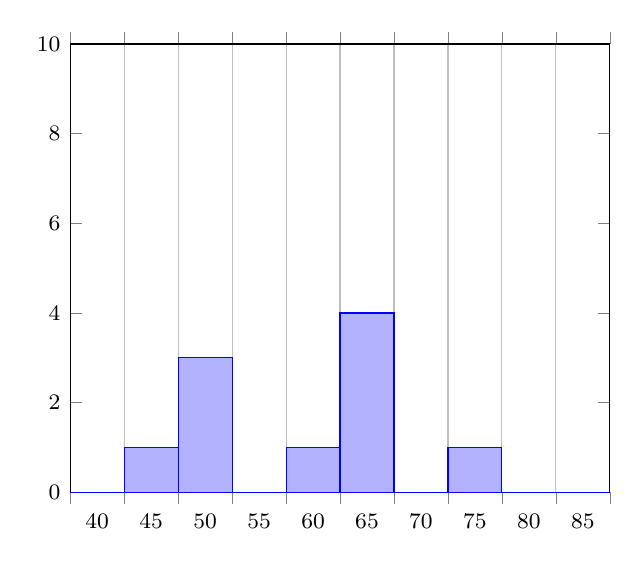
\begin{tikzpicture}
			\tikzstyle{every node}=[font=\footnotesize]
			\begin{axis}[ybar interval, ymin=0, ymax=10, xmin=40, xmax=90]
			\addplot coordinates {(40,0) (45,1) (50,3) (55,0) (60,1) (65,4) (70,0) (75,1) (80,0) (85,0) (90,0)};
			\end{axis}
			\end{tikzpicture}
		}
		\vspace{1cm}\\
		\textbf{Histograma de Censuras - Grupo 3}
		\resizebox{300px}{!}{
			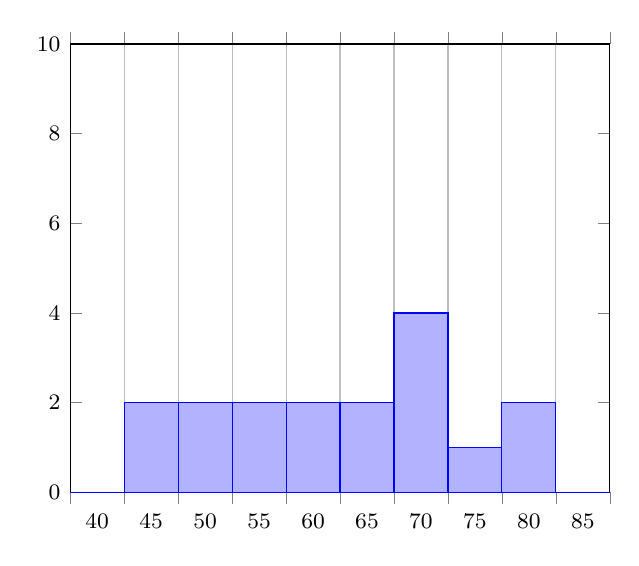
\begin{tikzpicture}
			\tikzstyle{every node}=[font=\footnotesize]
			\begin{axis}[ybar interval, ymin=0, ymax=10, xmin=40, xmax=90]
			\addplot coordinates {(40,0) (45,2) (50,2) (55,2) (60,2) (65,2) (70,4) (75,1) (80,2) (85,0) (90,0)};
			\end{axis}
			\end{tikzpicture}
		}
		\end{center}
		\vspace{1cm}
		As observações dos ocorrência de eventos do grupo de Estágio III de câncer de laringe se aproxima de uma distribuição normal. Assim, separar as censuras da ocorrência do falecimentos dos pacientes, as observações das censuras se distribuem igualmente entre as faixas etárias, desse modo, o evento morte parece ser responsável pela distribuição dos dados gerias se aproximarem de uma normal.
		\vspace{2cm}\\
		\begin{center}
		\textbf{Histograma de Eventos - Grupo 4}
		\resizebox{300px}{!}{
			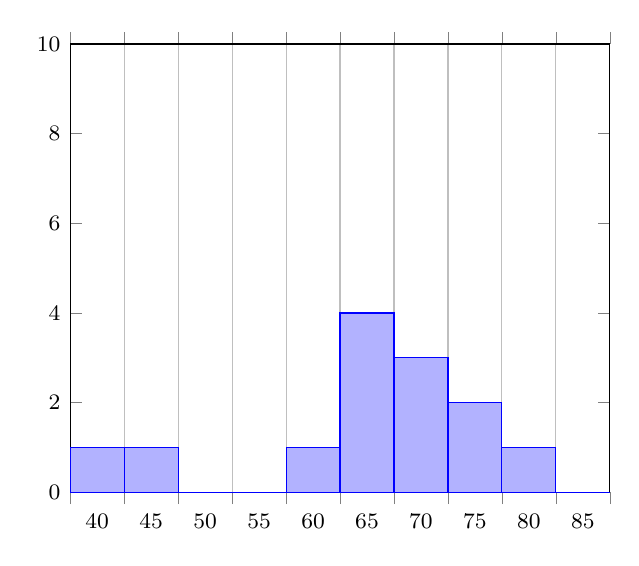
\begin{tikzpicture}
			\tikzstyle{every node}=[font=\footnotesize]
			\begin{axis}[ybar interval, ymin=0, ymax=10, xmin=40, xmax=90]
			\addplot coordinates {(40,1) (45,1) (50,0) (55,0) (60,1) (65,4) (70,3) (75,2) (80,1) (85,0) (90,0)};
			\end{axis}
			\end{tikzpicture}
		}
		\vspace{1cm}\\
		\textbf{Histograma de Sobrevivência - Grupo 4}
		\resizebox{300px}{!}{
			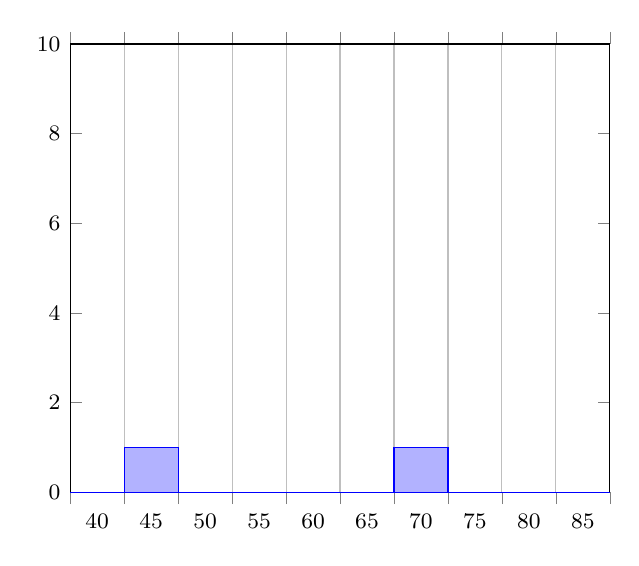
\begin{tikzpicture}
			\tikzstyle{every node}=[font=\footnotesize]
			\begin{axis}[ybar interval, ymin=0, ymax=10, xmin=40, xmax=90]
			\addplot coordinates {(40,0) (45,1) (50,0) (55,0) (60,0) (65,0) (70,1) (75,0) (80,0) (85,0) (90,0)};
			\end{axis}
			\end{tikzpicture}
		}
		\vspace{1cm}\\
		\textbf{Histograma de Censuras - Grupo 4}
		\resizebox{300px}{!}{
			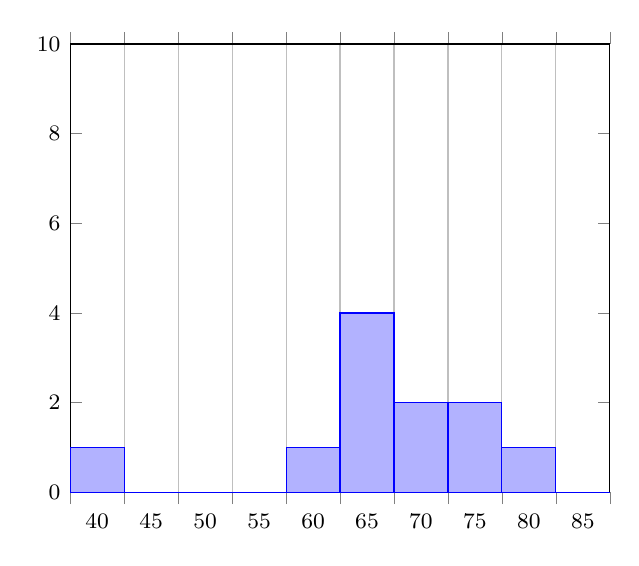
\begin{tikzpicture}
			\tikzstyle{every node}=[font=\footnotesize]
			\begin{axis}[ybar interval, ymin=0, ymax=10, xmin=40, xmax=90]
			\addplot coordinates {(40,1) (45,0) (50,0) (55,0) (60,1) (65,4) (70,2) (75,2) (80,1) (85,0) (90,0)};
			\end{axis}
			\end{tikzpicture}
		}	
	\end{center}
	\vspace{1cm}
	 Nas observações dos grupo de Estágio IV de câncer de laringe, os eventos de morte quase não foram observados, possivelmente, pelo número reduzido de pacientes em relação aos demais grupos. Assim, a curva geral é muito similar a curva de censuras.
	 \vspace{2cm}\\
	 \textbf{3. Ajuste de Modelos}\\
	 \vspace{1cm}\\
	 \textbf{3.1 Modelo 1}\\
	 \begin{center}
	 	\begin{tabular}{|c|c|c|c|c|c|}\hline
	 		& \textbf{Coef} & \textbf{Exp(Coef)} & \textbf{se(Coef)} & \textbf{z} & \textbf{Pr(>|z|)}\\ \hline   
	 		\textbf{Fator (Estágio 2)} & 0.06576 &  1.06797 & 0.45844 & 0.143 &   0.8859\\ \hline
	 		\textbf{Fator (Estágio 3)} & 0.61206 &  1.84423 & 0.35520 & 1.723 &   0.0849\\ \hline
	 		\textbf{Fator (Estágio4)} & 1.72284 &  5.60040 & 0.41966 & 4.105 & 4.04e-05 ***\\ \hline
	 	\end{tabular}
	 	\vspace{1cm}\\
	 	\begin{tabular}{|c|c|c|c|c|}\hline
	 		& \textbf{Exp(Coef)} & \textbf{Exp(-Coef)} & \textbf{IC$_{95\%}$ Inferior} & \textbf{IC$_{95\%}$ Superior}\\ \hline
	 		\textbf{Fator (Estágio 2)} & 1.068 & 0.9364 & 0.4348 & 2.623\\ \hline
	 		\textbf{Fator (Estágio 3)} & 1.844 & 0.5422 & 0.9193 & 3.700\\ \hline
	 		\textbf{Fator (Estágio 4)} & 5.600 & 0.1786 & 2.4604 & 12.748\\ \hline
	 	\end{tabular}
	 	\vspace{0.25cm}\\
	 	Concordância = 0.668  (se = 0.037 )\\
	 	Teste de Razão de Verossimilhança = 16.26  com 3 GL,   p=0.001\\
	 	Teste Wald = 18.95  com 3 GL,   p=3e-04\\
	 	Teste Logrank = 22.46  com 3 GL,   p=5e-05\\
	\end{center}
 	\vspace{1cm}
 	O modelo I considera apenas a variável Estágio da doença. Assim, submetendo o modelo aos testes, obtemos o valor de 0,668 como coeficiente de correlação de concordância. Já o Teste de Razão de Verossimilhança foi de 16,26 para um valor-p de 0,001. O teste Wald com coeficiente de 18,95 para um valor-p de 0,0003 e o teste de logrank com 22,46 de coeficiente um p valor de 0,00005, valores obtidos com 3 graus de liberdade e com significância estatística.\\
 	\vspace{2cm}\\
 	\textbf{3.2 Modelo 2}\\
 	\begin{center}
 		\begin{tabular}{|c|c|c|c|c|c|}\hline
 			& \textbf{Coef} & \textbf{Exp(Coef)} & \textbf{se(Coef)} & \textbf{z} & \textbf{Pr(>|z|)}\\ \hline   
 			\textbf{Fator (Estágio 2)} & 0.13856 & 1.14862 & 0.46231 & 0.300 &   0.764\\ \hline 
 			\textbf{Fator (Estágio 3)} & 0.63835 & 1.89335 & 0.35608 & 1.793 & 0.073\\ \hline 
 			\textbf{Fator (Estágio 4)} & 1.69306 & 5.43607 & 0.42221 & 4.010 & 6.07e-05 ***\\ \hline 
 			\textbf{Idade} & 0.01890 & 1.01908 & 0.01425 & 1.326 & 0.185\\ \hline 
 		\end{tabular}
 		\vspace{1cm}\\
 		\begin{tabular}{|c|c|c|c|c|}\hline
 			& \textbf{Exp(Coef)} & \textbf{Exp(-Coef)} & \textbf{IC$_{95\%}$ Inferior} & \textbf{IC$_{95\%}$ Superior}\\ \hline
 			\textbf{Fator (Estágio 2)} & 1.149 & 0.8706 & 0.4642 & 2.842\\ \hline
 			\textbf{Fator (Estágio 3)} & 1.893 & 0.5282 & 0.9422 & 3.805\\ \hline
 			\textbf{Fator (Estágio 4)} & 5.436 & 0.1840 & 2.3763 & 12.436\\ \hline
 			\textbf{Idade} & 1.019 & 0.9813 & 0.9910 & 1.048\\ \hline
 		\end{tabular}
 		\vspace{0.25cm}\\
 		Concordância = 0.682  (se = 0.039 )\\
 		Teste de Razão de Verossimilhança  = 18.07  com 4 GL,   p=0.001\\
 		Teste Wald = 20.82  com 4 GL,   p=3e-04\\
 		Teste Logrank = 24.33  com 4 GL,   p=7e-05\\
 	\end{center}
 	\vspace{1cm}
 	O modelo 2 acrescenta a variável Idade ao modelo. Ao rodarmos os teste no modelo, obtemos os valores de concordância de 0,682, no Teste de Razão de Verossimilhança, o valor-p continua igual a 0,001, mas com 4 graus de liberdade. Os teste de Wald e Logrank, ficam iguais 0,0003  e 0,00007 com 4 graus de liberdade, respectivamente. Demonstrando a significância da inclusão da variável.  
	\vspace{2cm}\\
	\textbf{3.3 Modelo 3}\\
 	\begin{center}
 			\begin{tabular}{|c|c|c|c|c|c|}\hline
 				& \textbf{Coef} & \textbf{Exp(Coef)} & \textbf{se(Coef)} & \textbf{z} & \textbf{Pr(>|z|)}\\ \hline
 				\textbf{Fator (Estágio 2)} & -7.946142 & 0.000354 & 3.678209 & -2.160 & 0.0307*\\ \hline
 				\textbf{Fator (Estágio 3)} & -0.122500 & 0.884706 & 2.468331 & -0.050 & 0.9604\\ \hline  
 				\textbf{Fator (Estágio 2)} & 0.846986 & 2.332605 & 2.425717 & 0.349 & 0.7270\\ \hline  
 				\textbf{Idade} & -0.002559 & 0.997444 & 0.026051 & -0.098 & 0.9218\\ \hline  
 				\textbf{Fator (Estágio 2):Idade} & 0.120254 & 1.127783 & 0.052307 & 2.299 & 0.0215*\\ \hline
 				\textbf{Fator (Estágio 3):Idade} & 0.011351 & 1.011416 & 0.037449 & 0.303 & 0.7618\\ \hline  
 				\textbf{Fator (Estágio 4):Idade} &  0.013673 & 1.013767 & 0.035967 & 0.380 & 0.7038\\ \hline
 			\end{tabular}
 			\vspace{1cm}\\
 			\begin{tabular}{|c|c|c|c|c|}\hline
 				& \textbf{Exp(Coef)} & \textbf{Exp(-Coef)} & \textbf{IC$_{95\%}$ Inferior} & \textbf{IC$_{95\%}$ Superior}\\ \hline
 				\textbf{Fator (Estágio 2)} & 0.000354 & 2824.6562 & 2.619e-07 & 0.4786\\ \hline
 				\textbf{Fator (Estágio 3)} &  0.884705 & 1.1303 & 7.011e-03 & 111.6467\\ \hline
 				\textbf{Fator (Estágio 4)} & 2.332605 & 0.4287 & 2.009e-02 & 270.7790\\ \hline
 				\textbf{Idade} & 0.997444 & 1.0026 & 9.478e-01 & 1.0497\\ \hline
 				\textbf{Fator (Estágio 2):Idade} & 1.127783 & 0.8867 & 1.018e+00 & 1.2495\\ \hline
 				\textbf{Fator (Estágio 3):Idade} & 1.011416 & 0.9887 & 9.398e-01 & 1.0884\\ \hline
 				\textbf{Fator (Estágio 4):Idade} & 1.013767 & 0.9864 & 9.448e-01 & 1.0878\\ \hline
 			\end{tabular}
 		\vspace{0.25cm}\\
 		Concordância = 0.694  (se = 0.039 )\\
 		Teste de Razão de Verossimilhança = 24.27  com 7 GL,   p=0.001\\
 		Teste Wald = 24.11  com 7 GL,   p=0.001\\
 		Teste Logrank = 28.59  com 7 df,   p=2e-04\\
 	\end{center}
	\vspace{1cm}
	O modelo 3 adiciona uma terceira variável teste de Concordância foi de 0,694, o maior entre todos os modelos. Por sua vez, o Teste de Razão de Verossimilhança foi de 24,27 com 7 graus de liberdade para um valor-p igual aos demais modelos, ou seja, 0,001. Ainda, no Teste Wald o coeficiente obtido foi 24,11 para um p-valor de 0,001 e no Teste Logrank o coeficiente foi 28,59 para um p-valor igual a 0,002 com 7 graus de liberdade. Todos os teste apresentando significância estatística. Portanto, a adição da variável tem significância ao modelo.\\
 	\vspace{2cm}\\
 	\textbf{4. Resíduos de Schoenfeld}\\
 	\vspace{1cm}\\
 	\textbf{4.1 Modelo 2}\\
 	\vspace{1cm}\\
 	\includegraphics[width=400px]{Gráfico 1.png}\\
 	\vspace{1cm}\\
 	O primeiro gráfico mostra interação do estágio da doença fator tempo com o estágio da doença, já o segundo gráfico introduz a variável Idade. O primeiro gráfico é apresenta uma homocedasticidade maior, o que causa uma variação menor ao longo do tempo que no segundo, indicando um ajuste melhor do valor de beta com base na suposição de proporcionalidade ao longo do tempo. Assim, o fator estágio da doença é mais propocional ao longo do tempo que o fator idade.
 	\vspace{2cm}\\
 	\textbf{4.2 Modelo 3}\\
 	\vspace{1cm}\\
 	\includegraphics[width=400px]{Gráfico 2.png}\\
 	\vspace{1cm}\\
 	Os valores dos betas ao longo do tempo para as variáveis Estágio e Estágio x Idade tem um formato similar, e sofrem menos variações se comparadas aos betas da variável Idade. 
 	\vspace{2cm}\\
 	\textbf{5. Estimativas de $\hat{S}_{0}(t)$ e $\hat{\Lambda}_{0}(t)$}\\
 	\begin{center}
 		\begin{tabular}{|c|c|c|}\hline
 			Tempos & S$_{0}$ & H$_{0}$\\ \hline
 			0.1 & 0.99377 & 0.00625\\ \hline
 			0.2 & 0.98739 & 0.01269\\ \hline
 			0.3 & 0.96737 & 0.03318\\ \hline
 			0.4 & 0.96039 & 0.04041\\ \hline
 			0.5 & 0.95319 & 0.04794\\ \hline
 			0.6 & 0.94596 & 0.05555\\ \hline
 			0.7 & 0.93875 & 0.06321\\ \hline
 			0.8 & 0.91713 & 0.08650\\ \hline
 			1.0 & 0.90154 & 0.10365\\ \hline
 			1.3 & 0.88552 & 0.12158\\ \hline
 			1.5 & 0.87745 & 0.13073\\ \hline
 			1.6 & 0.86907 & 0.14033\\ \hline
 			1.8 & 0.85231 & 0.15980\\ \hline
 			1.9 & 0.83549 & 0.17974\\ \hline
 			2.0 & 0.81848 & 0.20030\\ \hline
 			2.2 & 0.81848 & 0.20030\\ \hline
 			2.3 & 0.80945 & 0.21140\\ \hline
 			2.4 & 0.80004 & 0.22309\\ \hline
 			2.5 & 0.80004 & 0.22309\\ \hline
 			2.6 & 0.80004 & 0.22309\\ \hline
 			2.9 & 0.80004 & 0.22309\\ \hline
 			3.2 & 0.7765 & 0.24891\\ \hline
 			3.3 & 0.76923 & 0.26236\\ \hline
 			3.5 & 0.73805 & 0.30374\\ \hline
 			3.6 & 0.71695 & 0.33274\\ \hline
 			3.7 & 0.71695 & 0.33274\\ \hline
 			3.8 & 0.70498 & 0.34959\\ \hline
 		\end{tabular}
 		\hspace{0.5cm}
 		\begin{tabular}{|c|c|c|}\hline
 			Tempos & S$_{0}$ & H$_{0}$\\ \hline
 			4.0 & 0.66650 & 0.40572\\ \hline
 			4.3 & 0.65242 & 0.42707\\ \hline
 			4.5 & 0.65242 & 0.42707\\ \hline
 			4.8 & 0.65242 & 0.42707\\ \hline
 			5.0 & 0.63406 & 0.45561\\ \hline
 			5.1 & 0.63406 & 0.45561\\ \hline
 			5.3 & 0.61308 & 0.48925\\ \hline
 			5.5 & 0.61308 & 0.48925\\ \hline
 			5.9 & 0.61308 & 0.48925\\ \hline
 			6.0 & 0.59024 & 0.52723\\ \hline
 			6.1 & 0.59024 & 0.52723\\ \hline
 			6.2 & 0.56680 & 0.56775\\ \hline
 			6.3 & 0.54126 & 0.61386\\ \hline
 			6.4 & 0.48988 & 0.71360\\ \hline
 			6.5 & 0.46291 & 0.77022\\ \hline
 			6.7 & 0.46291 & 0.77022\\ \hline
 			7.0 & 0.43005 & 0.84384\\ \hline
 			7.4 & 0.39625 & 0.92571\\ \hline
 			7.5 & 0.39625 & 0.92571\\ \hline
 			7.6 & 0.39625 & 0.92571\\ \hline
 			7.8 & 0.35937 & 1.02341\\ \hline
 			8.0 & 0.35937 & 1.02341\\ \hline
 			8.1 & 0.35937 & 1.02341\\ \hline
 			9.3 & 0.35937 & 1.02341\\ \hline
 			9.6 & 0.35937 & 1.02341\\ \hline
 			10.1 & 0.35937 & 1.02341\\ \hline
 			10.7 & 0.35937 & 1.02341\\ \hline
 		\end{tabular}
 	\end{center}
 	\vspace{2cm}
 	\textbf{6. Curvas de Sobrevivência}
 	\vspace{1cm}\\
 	\includegraphics[width=400px]{Gráfico 3.png}\\
 	\vspace{1cm}\\
 	A Curva de Sobrevivência do Estágio I é ligeiramente diferente entre os grupos de 50 e 65 anos, tendo uma maior índice de eventos no primeiro grupo. Já para o Estágio II, a Curva de Sobrevivência é bastante discrepante em favor do grupo de pacientes com 50 anos, sendo a sobrevivência quase o dobro do grupo de 65 anos. Ja para os demais grupos, Estágio III e Estágio IV, em ambos os casos a distribuição é parecida tanto para pacientes com 50 anos como para pacientes com 65 anos. Assim, para esses Estágios da doença, a idade não parece ser um componente com grande influência na sobrevivência dos indivíduos. Em ambos os gráficos, os pacientes no Estágio II sobrevivem mais que os pacientes do Estágio I, que por sua vez, sobrevivem mais que os pacientes do Estágio III, que ainda apresentam maior sobrevivência que as pessoas com Estágio IV da doença.
 	\vspace{2cm}\\
 	\textbf{7. Curvas de Taxa de Falhas Acumulada}
 	\vspace{1cm}\\
 	\includegraphics[width=400px]{Gráfico 4.png}\\
 	\vspace{1cm}\\
 	Os gráficos das Taxas de Falha Acumuladas fornecem conclusões similares as obtidas pelos gráficos das Curvas de Sobrevivência, visto que, que são funções inversas. Assim, os Estágios I, III e IV, tem curvas similares entre si, enquanto o Estágio II, difere bastante entre as idades 50e 65 anos. Outro ponto importante, é a similaridade entre as Taxas de Falha Acumulada do Estágio I e Estágio II aos 65 anos. Portanto, a mudança no gráfico do Estágio II, sugere que a idade tem uma influência diretamente proporcional quando se trata desse estágio.    
 	\vspace{2cm}\\
 	\textbf{8. Códigos no R}\\
 	\vspace{1cm}\\
 	\# Importando bibliotecas\\
 	library('survival')\\
 	\vspace{0.25cm}\\
 	\# Definindo diretório de trabalho\\
 	setwd(getwd())\\
 	\vspace{0.25cm}\\
 	\# Leitura dos dados\\
 	laringe<-read.table("laringe.txt", h=T)\\
 	attach(laringe)\\
 	\vspace{0.25cm}\\
 	\# Ajuste de três modelos\\
 	\# Modelo 1\\
 	fit2<-coxph(Surv(tempos,cens) $\sim$ factor(estagio), data=laringe,
 	x = T, method="breslow")\\
 	summary(fit2)\\
 	fit2\$loglik\\
 	\vspace{0.25cm}\\
 	\# Modelo 2\\
 	fit3<- coxph(Surv(tempos,cens) $\sim$ factor(estagio)+ idade, data=laringe,
 	x = T, method="breslow")\\
 	summary(fit3)\\
 	fit3\$loglik\\
 	\vspace{0.25cm}\\
 	\# Modelo 3\\
 	fit4<-coxph(Surv(tempos,cens) $\sim$ factor(estagio) + idade + factor(estagio)*idade,
 	data=laringe, x = T, method="breslow")\\
 	summary(fit4)\\
 	fit4\$loglik\\
 	\vspace{0.25cm}\\
 	\# Resíduos de Schoenfeld, verificação da suposição de riscos proporcionais (Modelo fit 3)\\
 	resid(fit3,type="scaledsch")\\
 	cox.zph(fit3, transform="identity")\\
 	par(mfrow=c(1,2))\\
 	plot(cox.zph(fit3), xlab = "Tempo", ylab = c("Beta para o Fator Estágio", "Beta para o Fator Idade"))\\
 	mtext("Valores de Beta", side = 3, line = - 2, outer = TRUE)\\
 	\vspace{0.25cm}\\
 	\# Resíduos de Schoenfeld, verificação da suposição de riscos proporcionais (Modelo fit 4)\\
 	resid(fit4,type="scaledsch")\\
 	cox.zph(fit4, transform="identity")\\
 	par(mfrow=c(1,3))\\
 	plot(cox.zph(fit4), xlab = "Tempo", ylab = c("Beta para o Fator Estágio", "Beta para o Fator Idade", "Beta para o Fator Estágio x Idade"))\\
 	mtext("Valores de Beta", side = 3, line = - 2, outer = TRUE)\\
 	\vspace{0.25cm}\\
 	\# Estimando a função sobrevida e a função taxa de falha acumulada
 	Ht<-basehaz(fit4,centered=F)\\
 	tempos<-Ht\$time\\
 	H0<-Ht\$hazard\\
 	S0<- exp(-H0)\\
 	round(cbind(tempos, S0,H0),digits=5)\\
 	\vspace{0.25cm}\\
 	\# Gráfico curvas de sobrevivência por grau da doença e idade - 50 e 65 anos\\
 	fit4<-coxph(Surv(tempos,cens) ~ factor(estagio) + idade + factor(estagio)*idade,
 	data=laringe, x = T, method="breslow")\\
 	Ht<-basehaz(fit4,centered=F)\\
 	tempos<-Ht\$time\\
 	H0<-Ht\$hazard\\
 	S0<- exp(-H0)\\
 	round(cbind(tempos,S0,H0),digits=5)\\
 	tt<-sort(tempos)\\
 	aux1<-as.matrix(tt)\\
 	n<-nrow(aux1)\\
 	aux2<-as.matrix(cbind(tempos,S0))\\
 	S00<-rep(max(aux2[,2]),n)\\
 	for(i in 1:n){\\
 	if(tt[i]> min(aux2[,1])){\\
 	i1<- aux2[,1]<= tt[i]\\
 	S00[i]<-min(aux2[i1,2])}}\\
 	ts0<-cbind(tt,S00)\\
 	ts0\\
 	b<-fit4\$coefficients\\
 	id<-50\\
 	st1<- S00\^(exp(b[4]*id))                \# S(t|x) estágio I   e idade = 50 anos\\
 	st2<- S00\^(exp(b[1]+((b[4]+b[5])*id)))  \# S(t|x) estágio II  e idade = 50 anos\\
 	st3<- S00\^(exp(b[2]+((b[4]+b[6])*id)))  \# S(t|x) estágio III e idade = 50 anos\\
 	st4<- S00\^(exp(b[3]+((b[4]+b[7])*id)))  \# S(t|x) estágio IV  e idade = 50 anos\\
 	id<- 65\\
 	st11<- S00\^(exp(b[4]*id))               \# S(t|x) estágio I   e idade = 65 anos\\
 	st21<- S00\^(exp(b[1]+((b[4]+b[5])*id))) \# S(t|x) estágio II  e idade = 65 anos\\
 	st31<- S00\^(exp(b[2]+((b[4]+b[6])*id))) \# S(t|x) estágio III e idade = 65 anos\\
 	st41<- S00\^(exp(b[3]+((b[4]+b[7])*id))) \# S(t|x) estágio IV  e idade = 65 anos\\
 	par(mfrow=c(1,2))\\
 	plot(tt,st1,type="s",ylim=range(c(0,1)),xlab="Tempos",ylab="S(t|x)",lty=1)\\
 	lines(tt,st2,type="s",lty=2)\\
 	lines(tt,st3,type="s",lty=3)\\
 	lines(tt,st4,type="s",lty=4)\\
 	legend(0,0.2,lty=c(1,2,3,4),c("estágio I","estágio II","estágio III","estágio IV"),
 	lwd=1,bty="n",cex=0.7)
 	title("Idade = 50 anos")\\
 	plot(tt,st11,type="s",ylim=range(c(0,1)),xlab="Tempos",ylab="S(t|x)",lty=1)\\
 	lines(tt,st21,type="s",lty=2)\\
 	lines(tt,st31,type="s",lty=3)\\
 	lines(tt,st41,type="s",lty=4)\\
 	legend(0,0.2,lty=c(1,2,3,4),c("estágio I","estágio II","estágio III","estágio IV"),
 	lwd=1,bty="n",cex=0.7)
 	title("Idade = 65 anos")\\
 	\vspace{0.25cm}\\
 	\# Gráfico taxa de falha por grau da doença e idade (50 e 65 anos)
 	Ht1<- -log(st1)\\
 	Ht2<- -log(st2)\\
 	Ht3<- -log(st3)\\
 	Ht4<- -log(st4)\\
 	Ht11<- -log(st11)\\
 	Ht21<- -log(st21)\\
 	Ht31<- -log(st31)\\
 	Ht41<- -log(st41)\\
 	par(mfrow=c(1,2))\\
 	plot(tt,Ht1,type="s",ylim=range(c(0,4)),xlab="Tempos",ylab="Risco Acumulado",lty=1)\\
 	lines(tt,Ht2,type="s",lty=2)\\
 	lines(tt,Ht3,type="s",lty=3)\\
 	lines(tt,Ht4,type="s",lty=4)\\
 	legend(0.5,3.5, lty=c(1,2,3,4),c("estágio I","estágio II","estágio III","estágio IV"),
 	lwd=1,bty="n",cex=0.7)
 	title("Idade = 50 anos")\\
 	plot(tt,Ht11,type="s",ylim=range(c(0,4)),xlab="Tempos",ylab="Risco Acumulado",lty=1)\\
 	lines(tt,Ht21,type="s",lty=2)\\
 	lines(tt,Ht31,type="s",lty=3)\\
 	lines(tt,Ht41,type="s",lty=4)\\
 	legend(0.5,3.5, lty=c(1,2,3,4),c("estadio I","estágio II","estágio III","estágio IV"),
 	lwd=1,bty="n",cex=0.7)
 	title("Idade = 65 anos")\\
\end{document}